\documentclass[12pt,fullpage,letterpaper]{article}

\newenvironment{proof}{\noindent{\bf Proof:}}{\qed\bigskip}

\newtheorem{theorem}{Theorem}
\newtheorem{corollary}{Corollary}
\newtheorem{lemma}{Lemma} 
\newtheorem{claim}{Claim}
\newtheorem{fact}{Fact}
\newtheorem{definition}{Definition}
\newtheorem{assumption}{Assumption}
\newtheorem{observation}{Observation}
\newtheorem{example}{Example}
\newcommand{\qed}{\rule{5pt}{7pt}}

\newcommand{\assignment}[4]{
\thispagestyle{plain} 
\newpage
\setcounter{page}{1}
\noindent
\begin{center}
\framebox{ \vbox{ \hbox to 7in
{\bf CS466: Introduction to Bioinformatics \hfill #1}
\vspace{4mm}
\hbox to 6.28in
{\hspace{2.5in}\large\mbox{Problem Set #2}}
\vspace{4mm}
\hbox to 6.28in
{{\it Handed out: #3 \hfill Due: #4}}
}}
\end{center}
}


\newcommand{\handout}[3]{
\thispagestyle{plain} 
\newpage
\setcounter{page}{1}
\noindent
\begin{center}
\framebox{ \vbox{ \hbox to 6.28in
{\bf CS466: Introduction to Bioinformatics \hfill #1}
\vspace{4mm}
\hbox to 6.28in
{\hspace{2.5in}\large\mbox{#2}}
\vspace{4mm}
\hbox to 6.28in
{{\it Handed Out: #3 \hfill Name (NetID): \rule[-2pt]{4cm}{0.1pt} }}
}}
\end{center}
}


\newcommand{\assgsoln}[4]{
\thispagestyle{plain} 
\newpage
\setcounter{page}{1}
\noindent
\begin{center}
\framebox{ \vbox{ \hbox to 6.28in
{\bf CCS466: Introduction to Bioinformatics n \hfill #1}
\vspace{4mm}
\hbox to 6.28in
{\hspace{2.5in}\large\mbox{Problem Set #2 Solutions}}
\vspace{4mm}
\hbox to 6.28in
{{\it Handed Out: #3 \hfill Handed In: #4}}
}}
\end{center}
}


\newenvironment{algorithm}
{\begin{center}
\begin{tabular}{|l|}
\hline
\begin{minipage}{1in}
\begin{tabbing}
\quad\=\qquad\=\qquad\=\qquad\=\qquad\=\qquad\=\qquad\=\kill}
{\end{tabbing}
\end{minipage} \\
\hline
\end{tabular}
\end{center}}

\def\Comment#1{\textsf{\textsl{$\langle\!\langle$#1\/$\rangle\!\rangle$}}}





\oddsidemargin 0in
\evensidemargin 0in
\textwidth 6.5in
\topmargin -0.5in
\textheight 9.0in

\usepackage{hyperref}
\usepackage{float}
\usepackage{pdfpages}
\usepackage{textcomp}
\usepackage{mathtools}
\usepackage{algorithm}
\usepackage{array}
\usepackage{tabu}
\usepackage{changepage}
\usepackage{amsmath}
\usepackage{amssymb}
\usepackage[noend]{algpseudocode}
\usepackage{graphicx,url,epstopdf}
\usepackage{xcolor}
\usepackage{forest}
\makeatletter
\def\BState{\State\hskip-\ALG@thistlm}
\makeatother
\sloppy
\usepackage{colortbl}


\newcommand\tab[1][1cm]{\hspace*{#1}}

\begin{document}

% \answerstrue

\assignment{Name: Payal Mantri(payaljm2) \hspace{5cm}}{3}{October 26, 2022}{November 3, 2022}
% Fill in the above, for example, as follows:
% \solution{Joe Smith}{\today}{1}{Fall 2012}

\pagestyle{myheadings}  % Leave this command alone

\noindent\emph{Instructions:} This homework assignment consists of three questions worth a total of 50 points. 
In addition, Q2d and Q2e are worth an additional 10 bonus points.
\textbf{Do not forget to write your name at the top!}

\begin{enumerate}

\item[1.]  \textbf{RNA Secondary Structure} [15~points]

Consider the following RNA secondary structure. 
\begin{center}
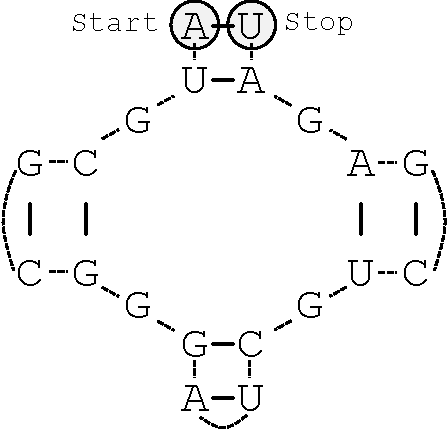
\includegraphics[width=.45\textwidth]{RNA-crop.pdf}
\end{center}
This is the optimal pseudoknot-free secondary structure for the RNA sequence $\mathbf{v} = \mathrm{AUGCGCGGGAUCGUCGAGAU}$, where only base pairings in $$\Gamma = \{ (A,U), (U,A), (G,C), (C,G)\}$$ receive a score of 1 (and the other base pairings have a score of 0).
We will represent this solution in two different ways. %reconstruct this solution by filling out the Nussinov dynamic programming table.

\begin{itemize}
\item[a.] Use the dot-parenthesis format represent the structure. [5~points]

\emph{Hint: } Number the bases from 1 to 20 in the figure.
\end{itemize}

\fbox{\parbox{1.11\linewidth}{
\begin{center}
    \begin{tabular}{|c|c|c|c|c|c|c|c|c|c|c|c|c|c|c|c|c|c|c|c|c|c|}
        \hline
          1 &2 &3  &4  &5  &6  &7  &8   & 9 & 10 & 11 & 12 & 13 & 14 & 15 & 16 & 17  & 18 & 19 & 20 \\
         \hline
         A & U & G & C & G & C & G & G & G & A & U & C & G & U & C & G & A & G & A & U\\
         \hline
        \hline
         &  &  &  &  &  &  &   &  &  &  &  &  &  &  &  &   &  &  & \\
         (  &(  &-  &(  &(  &)  &)   &-  &(  &(  &)  &)  &-  &(  &(  &)   &)  &-  &) &) \\
        
        \hline
    \end{tabular}
\end{center}
}}

% \clearpage
\newpage
\begin{itemize}
\item[b.] Recall the Nussinov algorithm, which was based on the following recurrence, where $s[i,j]$ indicates the maximum number of complementary base pairings in the sequence $v_i,\ldots,v_j$.
\begin{equation}
s[i,j] = \max
\begin{cases}
  0, & \mbox{if $i \ge j$,}\\
  s[i+1,j-1] + 1, & \mbox{if $i < j$ and $(v_i,v_j) \in \Gamma$,}\\
  s[i+1,j-1], & \mbox{if $i < j$ and $(v_i,v_j) \not \in \Gamma$,}\\
  s[i+1,j], & \mbox{if $i < j$,}\\
  s[i,j-1], & \mbox{if $i < j$,}\\
  \max_{i < k < j}\{s[i,k]+s[k+1,j]\}, & \mbox{if $i < j$.}
\end{cases}
\end{equation}
Represent the given optimal structure by performing a backtrace from cell $(1,n) = (1,20)$ in the following table.
% \textbf{Use directed arrows to illustrate transitions during the backtrace} (e.g.\ there is a directed arrow from $(1,20)$ to $(2,19)$).
\textbf{Only fill out the cells that correspond to the given structure.} [10~points]

\emph{Hint:} Cell $(1,20)$ has score $s[1,20] = 8$, corresponding to the eight complementary base pairings. Since $v_1$ and $v_{20}$ are paired up in the given structure, we move from $(1,20)$ to $(2,19)$. The latter cell has a score of $s[2,19] = 7$ complementary base pairings. These two cells have already been filled out in the table.
\end{itemize}
\end{enumerate}


\fbox{\parbox{1.1\linewidth}{
\begin{center}
\begin{tabular}{|c|c|c|c|c|c|c|c|c|c|c|c|c|c|c|c|c|c|c|c|c|}
\hline
& 1 & 2 & 3 & 4 & 5 & 6 & 7 & 8 & 9 & 10 & 11 & 12 & 13 & 14 & 15 & 16 & 17 & 18 & 19 &20\\ \hline
& A & U & G & C & G & C & G & G & G & A & U & C & G & U & C & G & A & G & A & U\\ \hline
1 A & 0 & & & & & & & & & & & & & & & & & & & \cellcolor{yellow}{8} \\ \hline
2 U & 0 & 0 & & & & & & & & & & & & & & & & & \cellcolor{yellow}{7} &  \\ \hline
3 G & &0 & 0 & & & &\cellcolor{yellow}{2} & & & & & & & & & &\cellcolor{yellow}{6} &\cellcolor{yellow}{6}  &  & \\ \hline
4 C & & &0 &0 & & &\cellcolor{yellow}{2} & & & & & & & & & & &  &  & \\ \hline
5 G & & & &0 &0 &\cellcolor{yellow}{1} & & & & & & & & & & & & &  & \\ \hline
6 C & & & & &0 &0 & & & & & & & & & & & & &  & \\ \hline
7 G & & & & & &0 &0 & & & & & & & & & & & &  & \\ \hline
8 G & & & & & & &0 &0 & & & & & & & & &\cellcolor{yellow}{4} & &  & \\ \hline
9 G & & & & & & & &0 &0 & & &\cellcolor{yellow}{2} & & & & &\cellcolor{yellow}{4} & &  & \\ \hline
10 A& & & & & & & & &0 &0 &\cellcolor{yellow}{1} & & & & & & & &  & \\ \hline
11 U& & & & & & & & & &0 &0 & & & & & & & &  & \\ \hline
12 C& & & & & & & & & & &0 &0 & & & & & & &  & \\ \hline
13 G& & & & & & & & & & & &0 &0 & & & &\cellcolor{yellow}{2} & &  & \\ \hline
14 U& & & & & & & & & & & & &0 &0 & & &\cellcolor{yellow}{2} & &  & \\ \hline
15 C& & & & & & & & & & & & & &0 &0 &\cellcolor{yellow}{1} & & &  & \\ \hline
16 G& & & & & & & & & & & & & & &0 &0 & & &  & \\ \hline
17 A& & & & & & & & & & & & & & & &0 &0 & &  & \\ \hline
18 G& & & & & & & & & & & & & & & & &0 &0 &  & \\ \hline
19 A& & & & & & & & & & & & & & & & & & 0& 0 & \\ \hline
20 U& & & & & & & & & & & & & & & & & & & 0 & 0 \\ \hline
\end{tabular}
\end{center}
}}



\newpage
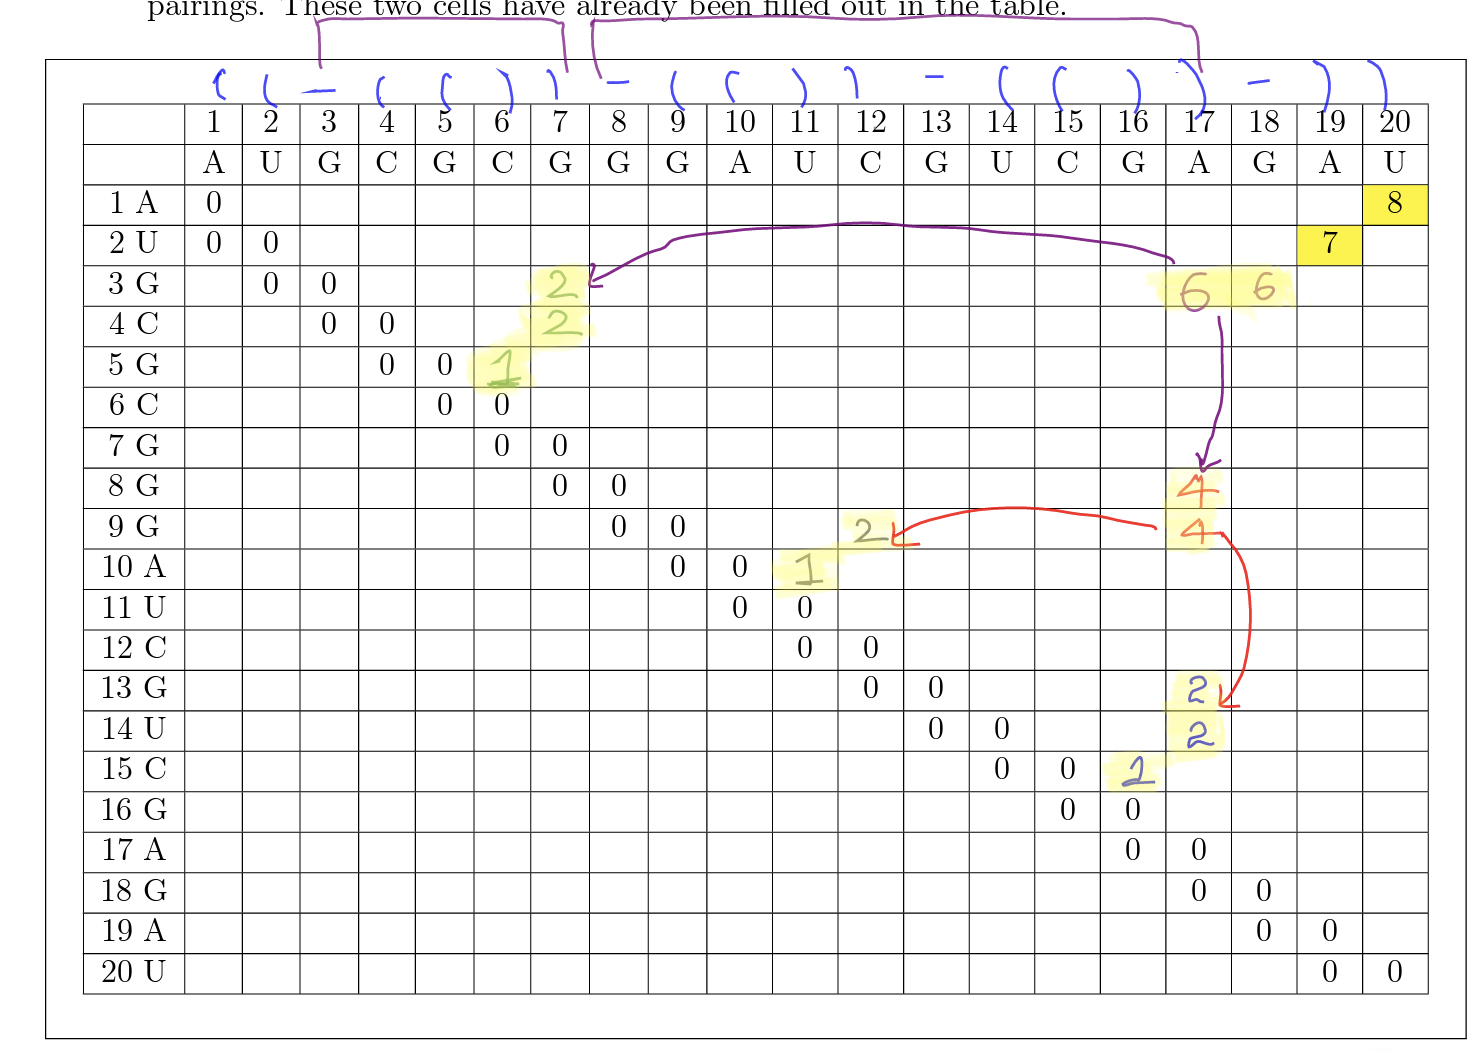
\includegraphics[scale=0.35]{9FF4ED5C-8163-46D7-AC61-E45FD06B7E6E.jpeg}
\clearpage
\begin{enumerate}
\item[2.] \textbf{Additive Phylogeny} [20 points]

\begin{enumerate}
\item Suppose you are working with a biological collaborator and they have obtained the sequences of the same gene from 5 different, but closely related, species.  They have done some initial analysis to compute pairwise distances between between the different species (maybe using something as simple as edit distance, or perhaps something more sophisticated).  These distances are shown in the table below.  

\begin{center}
\begin{tabular}{|c|ccccc|}
\hline
& a & b & c & d &e\\
\hline
a & 0 & 8 & 15 & 9 & 13\\
b & 8 & 0 & 5 & 10 & 11\\
c & 15 & 5 & 0 & 11 & 17\\
d & 9 & 10 & 11 & 0 & 3 \\
e & 13 & 11 & 17 & 3 & 0\\
\hline
\end{tabular}
\end{center}

Is the above distance matrix additive? Justify your answer. [5~points]



\fbox{\parbox{\linewidth}{
As per Four point Condition theorem\\
Every four leaves (quartet) can be labeled as (i,j, k, l) such that

\(d_{i,j}+d_{k,l} \le d_{i,k}+d_{j,l} = d_{i,l}+d_{j,k}\)\\
Let D be an n × n distance matrix. Matrix D is additive if and only if
the four point condition holds for every quartet  $ i,j, k, l  \in n^4$ \\ \\
We prove that given matrix D  is \textbf{not additive} by using contradiction. \\

Let us consider quartet a,b,c,d\\
$d_{a,b}+d_{c,d}$ = 8+11= 19\\
$d_{a, c}+d_{b,d}$ = 15+11 = 26\\
$d_{a,d}+d_{b,c}$ = 9+5 = 14 \\

For this quartet, the four point condition doesn't hold true , as there are no two sums whose value is equal to each other and greater than the third sum.\\\\
Since the condition doesn't hold true for atleast one of of the quartet, by method of contradiction, we can say that \textbf{D is not additive}.
\vspace{4cm}
}}


\clearpage

\item In class we considered the large additive distance phylogeny problem with $n=3$ sequences.

\begin{center}
    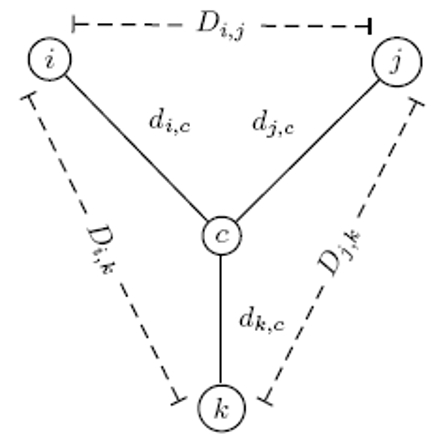
\includegraphics[width=.3\textwidth]{n_equals_3.png}
\end{center}

We derived $d_{i,c} = \frac{D_{i,j} - D_{j,k} + D_{i,k}}{2}$.
\textbf{Derive $d_{j,c}$ and $d_{k,c}$} in terms of $D_{i,j}$, $D_{i,k}$ and $D_{j,k}$.
Provide all intermediate steps.
[5~points]

\fbox{\parbox{\linewidth}{
We have\\
\begin{align}
    D_{i,j} = d_{i,c} +d_{j,c} \label{eq2}\\
    D_{i,k} = d_{i,c} +d_{k,c} \label{eq3}\\
    D_{j,k} = d_{j,c} +d_{k,c} \label{eq4}
\end{align}
\begin{enumerate}
    \item To derive $d_{j,c} $\\

    Adding equation 2 and 4 \\
    \begin{align*}
         D_{i,j}+D_{j,k}  &= d_{i,c} +d_{j,c} +  d_{j,c} +d_{k,c}\\
        D_{i,j}+D_{j,k} &= 2d_{j,c} +  (d_{i,c} +d_{k,c}) \\
        D_{i,j}+D_{j,k} & = 2d_{j,c} + D_{i,k} && \text{Using }\eqref{eq3} \\
        \intertext{ rearranging the terms above , we have } \\
        d_{j,c} &= \frac{D_{i,j} + D_{j,k} - D_{i,k}}{2}
    \end{align*}

        \item To derive $d_{k,c} $\\

    Adding equation 3 and 4 \\
    \begin{align*}
         D_{i,k}+D_{j,k}  &= d_{i,c} +d_{k,c} +  d_{j,c} +d_{k,c}\\
        D_{i,k}+D_{j,k} &= 2d_{k,c} +  (d_{i,c} +d_{j,c}) \\
        D_{i,k}+D_{j,k} & = 2d_{k,c} + D_{i,j} && \text{Using }\eqref{eq2} \\
        \intertext{ rearranging the terms above , we have } \\
        d_{k,c} &= \frac{D_{i,k} + D_{j,k} - D_{i,j}}{2} \\
    \end{align*}
\end{enumerate}

\vspace{0.25cm}
}}
 \clearpage
\item
How do you calculate the trimming parameter $\delta$ when constructing an additive phylogeny?  Explain using words and mathematical expressions, or provide pseudocode. As usual, pseudocode should contain initializations of variables and an explanation of what they represent. [10~points]

\emph{Hint:} 
A \textbf{hanging edge} of the triple $(A,B,C)$ of leaves is the edge $(B,P)$ connecting leaf $B$ and the first common vertex $P$ on the paths from $A$ to $C$ and from $B$ to $C$. 
The trimming parameter $\delta$ equals the length of the \textbf{shortest} hanging edge.



\fbox{\parbox{\linewidth}{

Given n × n distance matrix D = $[D_{i,j}]$, where $D_{i,j}$  represents distance between nodes  i and j

For every three leaf nodes triple $(i,j,k) \in D$,\\
    assume c as center point and calculate distance from each of node to c using following equations
   \[
 d_{i,c} = \frac{D_{i,j} - D_{j,k} + D_{i,k}}{2} \\\]
 \[d_{j,c} = \frac{D_{i,j} + D_{j,k} - D_{i,k}}{2}\\\]
 \[d_{k,c} = \frac{D_{i,k} + D_{j,k} - D_{i,j}}{2}\\
\]
Now find minimum value $min_{i,j,k} = min \{ d_{i,c},  d_{j,c},d_{k,c} \}$

This $min_{i,j,k}$ gives minimum value for triplet (i,j,k).
\\Calculate a minimum value from all the minimum of all possible triplets in D  to get delta. \\
\\
It can be represented using following way

\[ \delta = \min_{0 \le i<j<k<n} \{\min(d_{(i,c)} \ , d_{(j,c)}\ ,d_{(k,c)} )\}\]

\\For a n*n matrix , There ${n \choose 3}$ combinations of i,j,k . And we need to calculate 3 sums for each of these triple .\\
And to get minimum of all minimums ,we will run through array of size  ${n \choose 3}$\\
Hence total running time of algorithm is $O\left(  {n \choose 3}\right)$ which is $O(n^3)$
\vspace{5cm}
}}

\clearpage
\item Bonus question: Give a $3 \times 3$ matrix such that the matrix (i) is symmetric, (ii) has diagonal entries of $0$ and (iii) is NOT additive. If you think this is impossible, explain why. Otherwise, does your matrix satisfy the triangle equality? [5 points]

\fbox{\parbox{\linewidth}{
D=$ \begin{bmatrix}
0 & 2 & 5\\
2 & 0 & 1 \\
5 & 1 & 0 
\end{bmatrix}  $ \\

D  (i) is symmetric, (ii) has diagonal entries of $0$ and (iii) is NOT additive. \\
However D doesn't satisfy the triangle inequality  rule. 
\vspace{7cm}
}}
\clearpage
\item Bonus question: Give a $3 \times 3$ matrix such that the matrix (i) is symmetric, (ii) has diagonal entries of $0$, (iii) satisfies the triangle inequality and (iv) is NOT additive. If you think this is impossible, explain why. [5 points]

\fbox{\parbox{\linewidth}{
.It is impossible to construct a 3x3 matrix with the given conditions which is not additive . \\
Let i,j,k be nodes of matrix D =
$ \begin{bmatrix}
0 & D_{i,j} & D_{i,k} \\
D_{i,j} & 0 & D_{j,k} \\
D_{i,k} & D_{j,k} & 0 
\end{bmatrix}  $ \\
\\
We can see  D (i) is symmetric, (ii) has diagonal entries of $0$.
\\ Now assume D satisfies triangle inequality(the sum of any two distances is greater than third one) i.e 
\begin{align}
    D_{i,j}+ D_{i,k} > D_{j,k}\label{ref1}\\
    D_{i,k}+D_{j,k} > D_{i,j} \label{ref2}\\
    D_{i,j} + D_{j,k} > D_{i,k} \label{ref3}
\end{align}
Now we prove that it is impossible for D to  NOT be Additive matrix by contradiction. \\That is we prove that  D  is additive \\
We create a tree with c as center for the points i,j, k
\begin{center}
    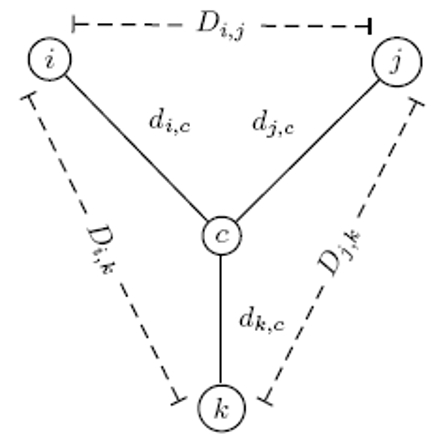
\includegraphics[width=.3\textwidth]{n_equals_3.png}
\end{center}

And we have 
 \begin{align}
 d_{i,c} = \frac{D_{i,j} - D_{j,k} + D_{i,k}}{2} \\
 d_{j,c} = \frac{D_{i,j} + D_{j,k} - D_{i,k}}{2}\\
 d_{k,c} = \frac{D_{i,k} + D_{j,k} - D_{i,j}}{2}
\end{align}
Now  for $ d_{i,c}$ is always positive as  from \eqref{ref1} $D_{i,j}+ D_{i,k} > D_{j,k}$. \\
Similarly $  d_{j,c} \ and \ d_{k,c}$ are also positive . And we have a edge-weighted tree T with i,j,k as leaves that best fits matrix D. \textbf{Thus D is additive.} \\
\\
Thus we can say that it is impossible to create a 3x3 matrix which satisfies all 4 conditions mentioned

}}

\end{enumerate}
\end{enumerate}


\clearpage
\begin{enumerate}

\item[3.] \textbf{Two-state Perfect Phylogeny} [15 points]

In this question we will consider a variant on the two-state perfect phylogeny problem called the \textit{Incomplete Directed Perfect Phylogeny Problem}.  
In this problem instead of observing a binary matrix $M$, where the $m$ rows are samples and the $n$ columns are characters (that are either expressed (1) or not expressed (0), you observe an incomplete matrix $M \in \{0,1,*\}^{m \times n}$.  In this matrix, $0$ and $1$ mean the same thing a previously, but an entry of $*$ indicates that the information was incomplete and we were unable to be measure that character in the corresponding sample.  The ``Directed'' part of this problem means that mutations are only ever gained (i.e. we only ever go from a 0 to a 1).  The following is an example of such a directed incomplete matrix $M$:

\begin{center}
\begin{tabular}{|c|ccccc|}
\hline
 & 1 & 2 & 3 & 4 & 5\\
 \hline
 a & 1& 1 & 0 & 0 & *\\
 b & 0 & * & 1 & 0 & *\\
 c & 1 & * & 0 & 0 & 1\\
 d & 0 & 0 & 1 & 1 & *\\
 e & 0 & 1 & 0 & 0 & *\\
 \hline
\end{tabular}
\end{center}

\begin{enumerate}
\item Fill in values to the above matrix such that it is compatible with a two-state perfect phylogeny (and construct the corresponding tree) or provide an argument as to why no such completion exists. [5~points]\\\\

\fbox{\parbox{\linewidth}{
The matrix that will be compatible with two-state perfect phylogeny 
\begin{center}
\begin{tabular}{|c|ccccc|}
\hline
 & 1 & 2 & 3 & 4 & 5\\
 \hline
 a & 1& 1 & 0 & 0 & 0\\
 b & 0 & 0 & 1 & 0 & 0\\
 c & 1 & 1 & 0 & 0 & 1\\
 d & 0 & 0 & 1 & 1 & 0\\\
 e & 0 & 1 & 0 & 0 & 0\\
 \hline
 \end{tabular}
 \end{center}

The tree for corresponding matrix is \\
\begin{center}
     \begin{forest}
for tree={circle,draw, l sep=25pt}
[ 
    [ , edge label={node[midway,left] {2}} 
      [,edge label={node[midway,left] {1}} 
       [a]
      [, edge label={node[midway, right] {5}}
      [b]]
    ] 
     
       [e]
      ]
    [ ,  edge label={node[midway,right] {3}} 
      [b] 
      [, edge label={node[midway,right] {4}} 
      [d]] 
      
  ] 
]
\end{forest}
\end{center}
\vspace{1cm}
}}
\clearpage

\item Suppose you are given an incomplete matrix $M \in \{0,1,*\}^{m \times n}$.  Give pseudocode for a brute force algorithm to determine whether or not $M$ admits a perfect phylogeny. Let $k$ be the number of missing entries. Give the running time of your algorithm.   [10~points]\\\\

\fbox{\parbox{\linewidth}{
Given there are k missing entries in the matrix. Each entry can take two possible values 0 or 1. \\
The idea is to generate all possible permutations of 0 and 1 of length k and use each permutation to check whether the matrix is perfect phylogeny \\
Label each missing entry a value i such that $0 \le i \le k-1$.
Generate all possible permutations C of 1s and 0s of length k in following manner \\
\[P_j= \{s_{i} | s_{i} = 0\ or \ 1 \ \& \  0 \le i \le k-1 \}  \quad | \  0 \le j \le 2^k-1\] 

\\For each permutations $P_j$,  generate a new matrix $D_{P,j}$ by filling missing entry labelled i as $i^{th}$ value in $C_j$
\begin{equation*}
D_{P,j} [a,b] = \begin{cases}
D[a][b] & a \le m , b\le n \  and \  D[a][b]  \in  \{0,1\}\\
P_j[i] &   \text{ where i is label of missing entry }
\end{cases}
\end{equation*}
Check if $D_{P,j}$ is a perfect phylogeny  by using the Two-State Perfect Phylogeny algorithm as discussed in class.\\
If for any $j \in 0 \le j \le a^k-1$ Matrix $D_{P,j}$ satisfies the problem, Then we can say that given Matrix M  admits a perfect phylogeny .\\

\\
\textbf{Running time}
there $2^k$ possible permutations for k missing entries. 
for each combination, to check whether a matrix$ M \in \{0, 1\}^{m,n}$ admits perfect phylogeny takes O(m*n) time .\\ 

Hence total running time is $O(2^k  mn)$
\vspace{3cm}
}}

\end{enumerate}
\end{enumerate}

\end{document}
